\documentclass[11pt]{article}
\usepackage{amsfonts}
\usepackage{amsmath}
\usepackage{multicol}
\usepackage[utf8x]{inputenc}
\usepackage{graphicx}
\usepackage{geometry}
\geometry{a4paper, total={170mm, 237mm}, left=20mm, top=20mm}
 
\title{ {\Large \textbf{DÉMONSTRATION AUTOMATIQUE EN COQ}} }
\date{}
\author{Quentin Garchery}

\setlength{\parindent}{0cm}



\usepackage{listings}
\usepackage{color}


\lstdefinelanguage{coq}
{morekeywords={[2]apply,eapply,reflexivity, match, with, end, constr, let, in, forall, change, rewrite, auto, simpl, induction, revert, intro, assumption, split, inversion, destruct, trivial},
keywordstyle={[2]\color{dkblue}},
sensitive=true,
}
\lstset{emph={Lemma, Theorem, Proposition, Qed, Proof, Inductive, Definition, Fixpoint, Ltac, Hint, Resolve, Require, Import, Open, Scope}, emphstyle={\color{mauve}\bf}
}
\definecolor{dkblue}{rgb}{0,0,0.6}
\definecolor{dkgreen}{rgb}{0,0.6,0}
\definecolor{gray}{rgb}{0.5,0.5,0.5}
\definecolor{mauve}{rgb}{0.58,0,0.82}

\lstset{frame=tb,
  language=coq,
  aboveskip=3mm,
  belowskip=3mm,
  showstringspaces=false,
  columns=flexible,
  basicstyle={\small\ttfamily},
  numbers=none,
  numberstyle=\tiny\color{gray},
  keywordstyle=\color{blue},
  commentstyle=\color{dkgreen},
  stringstyle=\color{mauve},
  breaklines=true,
  breakatwhitespace=true,
  tabsize=3
}



\begin{document}




\maketitle
\thispagestyle{empty}

\begin{center}
\normalsize sous la direction de \\

\vspace{3mm}

\begin{multicols}{2}
\large Chantal Keller \\
Maître de Conférences\\
Université Paris-Sud \\

\large Valentin Blot \\
Post-doctorant\\
Université Paris-Sud
\end{multicols}

\vspace{7mm}

\Large{Stage au LRI, Paris-Saclay\\
Université Paris-Sud / CNRS \\}

\vspace{5mm}

\normalsize Mars-Août 2018

\end{center}


\vspace{2cm}


\section{Fiche de synthèse}

\subsection{Contexte général: méthodes formelles}

Les méthodes formelles rassemblent différents logiciels formels qui permettent de formuler des propriétés mathématiques puis de les vérifier. La validité du résultat ne dépend alors que de ce logiciel de vérification. C'est dans ce cadre que G. Gonthier et B. Werner ont prouvé, en Coq, le théorème des quatre couleurs.\\

Les méthodes formelles s'étendent à la preuve de programme: il s'agit alors de vérifier qu'un programme correspond à sa spécification. Cela permet d'augmenter la robustesse et la fiabilité du programme certifié. C'est notamment le cas de Compcert \cite{compcert} qui est un compilateur de code C qui a été certifié en Coq par X. Leroy. L'importance de la correction des logiciels est mise en avant dans le cas des systèmes critiques. En effet, le premier lancement d'Ariane 5 (1996) s'est soldé par un échec dû à un bug logiciel. 

\subsection{Problème étudié}

Parmi ces logiciels formels, on s'intéressera aux assistants de preuves (\ref{assistants}) et aux prouveurs automatiques (\ref{prouveurs}) et plus particulièrement aux interfaces entre un assistant de preuve et différents prouveurs automatiques.  De telles interfaces permettent d'améliorer l'automatisation de l'assistant de preuve considéré. En effet, les preuves générées automatiquement par les prouveurs sont ensuite utilisées pour créer des preuves dans l'assistant de preuve. Cette approche est utilisée par Coqhammer \cite{coqhammer} pour Coq et par Sledgehammer \cite{sledgehammer_manual} pour Isabelle. \\
Pendant mon stage, j'ai travaillé sur SMTCoq qui sert aussi d'interface à différents prouveurs automatiques mais qui a la particularité de reconstruire fidèlement, en Coq, les preuves générées par les prouveurs automatiques. Cette approche permet de vérifier les certificats fournis par les prouveurs et donc d'augmenter la confiance que l'on a dans ces outils.\\

Nous aimerions que le développement à l'aide de cette automatisation soit adapté aux assistants de preuves: les preuves sont modulaires et peuvent reposer sur des lemmes précédemment démontrés. Nous voudrions aussi pouvoir formaliser une théorie en partant des axiomes de celle-ci puis démontrer automatiquement de nouvelles propriétés de cette théorie.

\subsection{Contribution proposée}

Pendant mon stage, je me suis attaché à améliorer l'expressivité de SMTCoq de ce point de vue là. J'ai donc rajouté la possibilité de transmettre à SMTCoq des axiomes ou des lemmes déjà démontrés. Cet ajout s'est traduit par une extension de la logique utilisée et se retrouve dans toutes les étapes intermédiaires de SMTCoq, étapes j'ai étendues en conséquence.  Cet aspect est original: la technique d'encodage des instanciations des lemmes que j'ai utilisée (\ref{processing_forallinst}) permet d'alléger la suite de la vérification. Enfin, j'ai automatisé le procédé de vérification final afin de préserver la facilité d'utilisation de SMTCoq.


\subsection{Arguments en faveur de la validité de la contribution}

En plus des tests présents dans SMTCoq initialement, le code final passe d'autres tests pour s'assurer du gain d'expressivité dû au rajout des lemmes et des quantificateurs. J'ai, par exemple, pu vérifier des propriétés, automatiquement et dans Coq, en théorie des groupes, dans une théorie formalisant les listes d'entiers, sur des fonctions définies récursivement, etc. \\ 
D'autre part, ma contribution respecte le principe sceptique de SMTCoq (\ref{sceptique_autarcique}), le développement et le calcul sont faits principalement en Ocaml, en dehors de l'assistant de preuve. Cet aspect donne une meilleure robustesse à SMTCoq face aux changements internes des prouveurs automatiques.


\subsection{Bilan et perspectives}\label{persp}

Un des buts que l'on souhaite poursuivre est de certifier le logiciel de vérification Why3 \cite{why3_intro}. Puisque Why3 utilise des prouveurs automatiques, il faut alors pouvoir certifier les démonstrations faites par ces prouveurs. Ce sujet est lié à celui de ma thèse intitulée "Certification de la génération et la transformation d'obligations de preuves" encadrée par Claude Marché, Chantal Keller et Andrei Paskevich. À cette occasion, j'utiliserai SMTCoq et je profiterai de l'amélioration de son expressivité due à mon stage. Je pourrai l'améliorer encore afin d'accepter des quantificateurs dans n'importe quelle position dans la formule.\\
L'expressivité peut également être améliorée en considérant les termes concrets du type des propositions dans Coq en plus de ceux du type des booléens. \\
On pourrait aussi utiliser des méthodes de \textit{machine learning} pour sélectionner les lemmes à envoyer au prouveur automatique comme c'est fait dans Coqhammer et Sledgehammer \cite{hol_selector, coqhammer}. L'avantage étant qu'avec des lemmes pertinents et en petit nombre le prouveur automatique trouve plus rapidement et plus souvent la preuve du théorème en question.\\

Ces améliorations de l'expressivité et de l'efficacité combinées avec la facilité d'utilisation et la robustesse de SMTCoq ont pour objectifs d'en faire un outil accessible et de généraliser son utilisation dans les projets développés en Coq.



\newpage
\section{Logiciels utilisés}

\subsection{Assistants de preuve}\label{assistants}

Les assistants de preuves sont des outils puissants qui permettent d'exprimer des théorèmes complexes puis de les vérifier de manière interactive. Ils proposent à un utilisateur de formuler son problème puis de le démontrer, le rôle principal de l'assistant de preuve étant alors de vérifier que la preuve fournie est correcte. Pour une propriété donnée, l'utilisateur doit donc fournir une preuve parfaitement rigoureuse et exhaustive de la propriété ce qui peut rendre le processus de vérification long et fastidieux. La confiance accordée à ces outils dépend de la compréhension que l'on peut avoir dans son noyau, étant donné que c'est la partie sur laquelle repose la vérification. Cette compréhension est facilitée lorsque l'implantation de la logique de ce noyau est de taille réduite. \\

Dans la suite nous utiliserons Coq comme assistant de preuve. La logique de son noyau se fonde sur le calcul des constructions inductives \cite{coq_intro}. La sémantique du langage n'est pas donnée en détail dans ce rapport mais les aspects importants seront précisés au moment de leur utilisation. La partie \ref{coq} introduit deux techniques d'utilisation de Coq. 

\subsection{Prouveurs automatiques}\label{prouveurs}

Les prouveurs automatiques, quant à eux, ne demandent pas de preuves de la part de l'utilisateur. L'effort de certification est alors réduit à la formalisation du problème et dans certains cas le prouveur donne une trace de son exécution appelée certificat. En contrepartie, la logique d'un prouveur automatique est plus limitée et/ou la réponse en temps fini n'est pas garantie.\\

Nous utiliserons différents prouveurs automatiques (voir partie \ref{fonctionnement_prouveurs}), de différents types, à savoir: 
\begin{itemize}
    \item zChaff, un prouveur SAT
    \item veriT, un prouveur SMT.
\end{itemize}


\subsection{SMTCoq}

Une interface entre assistant de preuve et prouveurs automatiques telle que SMTCoq offre les avantages décrits ci-dessus des deux types de logiciels formels. Un autre avantage de SMTCoq est sa modularité: il est en effet possible de rajouter d'autres prouveurs automatiques, ceux-ci n'étant pas nécessairement du même type (prouveurs SAT/SMT) et n'ayant pas nécessairement le même format d'entrée ni le même format de sortie. \\

Pendant ce stage j'ai travaillé sur SMTCoq. J'ai notamment eu l'occasion de modifier le code du projet qui est actuellement développé par Chantal Keller en collaboration avec l'université de l'Iowa. \\

Les fragments de code Coq fournis sont compilables lorsqu'ils sont chargés dans l'environnement de SMTCoq. Il faut donc les préfacer par
\begin{lstlisting}[frame=single]
  Require Import SMTCoq Bool.
  Open Scope Z_scope.
\end{lstlisting}
Cela requiert l'installation de SMTCoq, disponible sur \textit{github.com/smtcoq/smtcoq}.


\newpage

\section{Techniques de preuves en Coq} \label{coq}

Cette partie présente deux techniques de preuves en Coq qui peuvent être combinées: la réflexion calculatoire et la réification. Ces techniques sont au coeur du fonctionnement de SMTCoq.


\subsection{Réflexion calculatoire}

Pour définir de nouveaux termes en Coq, on peut utiliser les constructions inductives et les définitions. Nous allons voir que la réflexion calculatoire n'est possible que dans le second cas. Nous commençons par détailler les constructions inductives, ce qui permettra de mettre en avant cette différence.

\subsubsection{Constructions inductives}

Prenons l'exemple des formules conjonctives: 

\begin{lstlisting}[frame=single]
Inductive AndTree :=
  Bool (_ : bool)
| And (_ _: AndTree).
\end{lstlisting}

et définissons un type inductif qui donne son évaluation: 

\begin{lstlisting}[frame=single]
Inductive Evaluation : AndTree -> bool -> Prop :=
  EvalBool b :
    Evaluation (Bool b) b
| EvalAnd b1 b2 b3 t1 t2 :
    Evaluation t1 b1 -> Evaluation t2 b2 -> b1 && b2 = b3 ->
    Evaluation (And t1 t2) b3.
\end{lstlisting}
$Evaluation \, t \, b$ signifie que l'arbre $t$ s'évalue en un booléen $b$. Cette définition suit la définition des formules conjonctives. En effet, il y a bien deux cas, $EvalBool$ pour les feuilles de l'arbre et $EvalAnd$ pour les noeuds. Le cas $EvalAnd$ s'explique ainsi: si $t1$ s'évalue en $b1$ et $t2$ s'évalue en $b2$ alors $And \, t1 \, t2$ s'évalue en $b1\,\&\&\,b2$.  On a utilisé la fonction Coq $andb$ notée $\&\&$ qui implémente la conjonction booléenne.

On peut alors faire des preuves sur les éléments de ce type inductif: 
\begin{lstlisting}[frame=single]
Definition t := And (And (Bool true) (Bool false)) (And (Bool true) (Bool true)).

Lemma Eval_t_false : Evaluation t false.
Proof.
  eapply EvalAnd ; [
    eapply EvalAnd ; [ apply EvalBool | apply EvalBool | reflexivity ]
  | eapply EvalAnd ; [ apply EvalBool | apply EvalBool | reflexivity ]
  | reflexivity ].
Qed.
\end{lstlisting}

\subsubsection{Définitions en Coq et convertibilité}

La réflexion calculatoire repose sur la convertibilité de deux termes: deux termes sont convertibles lorsqu'ils se réduisent vers un même terme. Aussi, à chaque nouvelle définition, la nouvelle constante qui est définie est convertible à sa définition. \\

Plutôt que d'utiliser un prédicat qui prend une formule conjonctive $t$ et un booléen $b$, et qui vérifie que $t$ s'évalue en $b$, on peut utiliser une fonction récursive qui calcule l'évaluation et combiner cette fonction récursive avec le prédicat de l'égalité. On peut ensuite montrer que les deux formalisations sont bien équivalentes.  
\begin{lstlisting}[frame=single]
Fixpoint evaluation (t : AndTree) :=
  match t with
    Bool b => b
  | And t1 t2 => evaluation t1 && evaluation t2
  end.
  
Proposition Eval_eq_eval t b :
  Evaluation t b <-> evaluation t = b.
\end{lstlisting}

L'avantage de cette nouvelle définition de l'évaluation est que, grâce à la convertibilité de $evaluation$ avec sa définition, on a une preuve triviale de la propriété.
\begin{lstlisting}[frame=single]
Lemma eval_t_false : evaluation t = false.
Proof.
  reflexivity.
Qed.
\end{lstlisting}

En effet, en notant $a \equiv b$ lorsque $a$ est convertible à $b$, on a:
\begin{align*}
  evaluation \,\,t \equiv \,\, &evaluation\,\, (And \,\,(Bool \,\,true) \,\,(Bool \,\,false)) \,\,\&\& \,\, \\
  \,\, &evaluation\,\, (And \,\,(Bool\,\, true) \,\,(Bool\,\, true)) \\
  \equiv \,\, &(evaluation \,\,(Bool \,\,true) \,\,\&\&\,\, evaluation \,\,(Bool \,\,false)) \,\,\&\&\,\, \\
  &(evaluation\,\, (Bool \,\,true) \,\,\&\&\,\, evaluation \,\,(Bool\,\, true)) \\
  \equiv \,\, &(true \,\,\&\&\,\, false) \,\,\&\&\,\, (true \,\,\&\&\,\, true) \\
  \equiv\,\, &false \,\,\&\&\,\, (true \,\,\&\&\,\, true) \\
  \equiv\,\, &false
\end{align*}  

Ce fonctionnement peut être exploité pour construire des preuves qui reposent sur un calcul de convertibilité de termes Coq.


\subsection{Réification} \label{reification}

\subsubsection{\textit{Embeddings}}

La réification est le fait de passer d'un \textit{shallow-embedding} à un \textit{deep-embedding}. \\

Dans le cas du \textit{deep-embedding}, un terme est représenté dans un nouvel AST ce qui met en évidence sa structure. À l'inverse, un \textit{shallow-embedding} du même terme est traduit directement vers sa valeur dans le langage cible. \\

Reprenons l'exemple des formules conjonctives et considérons la formule $ u = (b_1 \,\&\, b_2) \,\&\, (b_3 \,\&\, b4)$. À l'instar de la section précédente, le \textit{deep-embedding} de $u$ est donné dans le type $AndTree$:
\[And\,(And\,(Bool\,b1)\,(Bool\,b2))\,(And\,(Bool\,b3)\,(Bool\,b4))\] 
et son \textit{shallow-embedding} peut être donné en utilisant la conjonction booléenne de Coq: 
\[(b1\,\&\&\,b2)\,\&\&\,(b3\,\&\&\,b4) \]

Dans la suite, on s'intéresse au problème de mettre des formules booléennes conjonctives en forme de peigne. Avec $b_1, b_2, b_3, b_4$ des termes de type $bool$, on veut, par exemple, pouvoir passer de: 
\begin{center}
$ u = (b_1 \,\&\&\, b_2) \,\&\&\, (b_3 \,\&\&\, b4)$ \hspace{1cm} à   \hspace{1cm}  $u' = b_1 \,\&\&\, (b_2 \,\&\&\, (b_3 \,\&\&\, b4)) $
\end{center}

Pour cela, on a besoin de récupérer la structure du booléen $u$, c'est l'étape de réification. Il s'agit donc de construire, à partir de $u$, un terme du type $AndTree$ qui a la même structure que $u$.

\subsubsection{Méthodes}

Il n'est pas possible d'écrire en Coq une fonction qui détermine la forme conjonctive d'un argument booléen. En effet, le type $bool$ n'ayant que deux constructeurs ($true$ et $false$), inspecter par \textit{pattern-matching} nous donnera un de ces deux constructeurs.\\

Une solution est d'étudier la structure du terme en question à partir de sa représentation Ocaml sous-jacente. C'est l'approche utilisée par SMTCoq. \\

Il est aussi possible d'utiliser des tactiques qui renvoient un terme. Dans le cas des formules conjonctives, on définit:

\begin{lstlisting}[frame=single]
Ltac reify A :=  match A with
  | andb ?X ?Y => let rx := reify X in
                    let ry := reify Y in
                    constr:(And rx ry)
  | ?X => constr:(Bool X) end.

\end{lstlisting}

Le terme $u = (b1\,\&\&\,b2)\,\&\&\,(b3\,\&\&\,b4)$ réifié donne bien 
\[And\,(And\,(Bool\,b1)\,(Bool\,b2))\,(And\,(Bool\,b3)\,(Bool\,b4))\] 
et on notera que l'évaluation de ce nouveau terme est égale à $u$.



\subsubsection{Intérêt et exemple d'utilisation} \label{interet_reification}

L'intérêt de la réification est que la structure du terme réifié est mise en évidence. Il devient alors possible de manipuler explicitement cette structure. \\

Par exemple, sur le type $AndTree$, il est possible de définir une fonction $peigne$ qui renvoie l'arbre en argument mis sous forme de peigne. Le théorème de correction de cette fonction établit que 
\[ \forall t \in AndTree, \, evaluation \, (peigne \, (t)) = evaluation (t) \]

Ce théorème de correction n'est applicable que si on a un terme de la forme $evaluation \, (x)$, forme que l'on peut obtenir en remarquant que pour tout terme booléen $b$, l'évaluation de la réification de $b$ est convertible à $b$.\\

En combinant tous ces résultats, on peut définir une tactique $peignify$ qui met les formules conjonctives en forme de peigne. Cette tactique permet par exemple de démontrer le lemme suivant: 

\begin{lstlisting}[frame=single]
Lemma peigne4 b1 b2 b3 b4:
  (b1 && b2) && (b3 && b4) = b1 && ((b2 && b3) && b4).
Proof.
  peignify. reflexivity.
Qed.
\end{lstlisting}
Cette preuve a un contenu calculatoire: le calcul de la fonction $peigne$ sur la réification du terme $u$ de type $bool$. Pour le code complet de cette partie, voir l'annexe A, la preuve de correction est inspirée de \cite{coq_intro}, section 3.3.


\newpage
\section{Prouveurs automatiques} \label{fonctionnement_prouveurs}

\subsection{Utilisation par SMTCoq}

Différents prouveurs automatiques sont mis à la disposition de l'utilisateur de SMTCoq. Parmi ceux-ci, on trouve des prouveurs SAT, des prouveurs qui résolvent des problèmes de satisfiabilité de formules booléennes ainsi que des prouveurs SMT que nous détaillons dans cette partie. \\ 

Pour SMTCoq, les prouveurs automatiques sont vus comme des boîtes noires qui résolvent des problèmes logiques. Plus précisément, SMTCoq interagit avec un prouveur automatique en traduisant le problème dans un format reconnu par celui-ci (\ref{smt-lib}) puis en interprétant sa réponse (\ref{sortie}). Ce fonctionnement est un des intérêts de l'approche sceptique (\ref{sceptique_autarcique}).

\subsection{Prouveurs SMT} \label{smt}

Expliquons succinctement le fonctionnement d'une version de l'algorithme DPLL \cite{dpll}. Nous ne considérerons que la théorie LIA, c'est-à-dire qu'en plus des connecteurs logiques, la théorie contient les entiers et les symboles d'addition, de soustraction et d'inégalité. On prend en exemple le problème qu'on appellera $lia5$ et qui consiste à satisfaire la formule $((x + y \leq -3 \wedge y \geq 0) \vee x \leq -3) \wedge x \geq 0$ où $x$ et $y$ sont des entiers. \\

L'algorithme commence par identifier les atomes, c'est-à-dire les sous-formules spécifiques à la théorie LIA. Dans notre exemple cela revient à poser 
\begin{align*}
a &= (x + y \leq -3) \\
b &= (y \geq 0) \\
c &= (x \leq -3) \\
d &= (x \geq 0)
\end{align*}

et à chercher si la formule  $((a \wedge b) \vee c) \wedge d$ est satisfiable. Cette étape peut être suivie par une transformation de Tseitin (\ref{tseitin}) afin d'obtenir un problème en Forme Normale Conjonctive (CNF) qui est le format de prédilection des prouveurs SAT. \\

Ensuite, l'algorithme DPLL répète les étapes suivantes:
\begin{itemize}
\item Appeler un prouveur SAT sur l'ensemble des formules (dans l'exemple on commence avec une seule formule). Si ce n'est pas satisfiable, alors l'algorithme répond que le problème n'est pas satisfiable.
\item Sinon, le prouveur SAT donne une instanciation qui satisfait toutes les formules. Dans l'exemple, une telle instanciation pourrait être:
  $a \, \wedge\,\neg b \, \wedge c\, \wedge \,d$,
ce qui signifie que toutes les variables booléennes sont à $true$ sauf $b$ qui est à $false$.
\item Vérifier que l'instanciation est valide dans les théories. Si c'est le cas, l'algorithme renvoie que le problème est satisfiable.
\item Sinon, rajouter la négation de l'instanciation à la liste des formules et recommencer. C'est le cas de notre exemple: il n'est pas possible, dans la théorie LIA, d'avoir à la fois $x \leq -3$ et $x \geq 0$. À la fin de cette étape, le problème est donc ramené à la satisfiabilité des deux formules suivantes:
  \begin{align*}
    ((a \wedge b) \vee c) \wedge d \\
    \neg a \vee b \vee \neg c \vee \neg d.
  \end{align*}
\end{itemize}

Cet algorithme termine puisque qu'à chaque répétition des étapes ci-dessus une nouvelle instanciation des atomes n'est plus possible et qu'il y a un nombre fini de telles instanciations. 

\subsection{Format d'entrée, le langage SMT-LIB} \label{smt-lib}

Le langage SMT-LIB a vocation à être un format d'entrée commun à différents prouveurs SMT tels que veriT. Ce langage offre donc un cadre pour faire des comparaisons de prouveurs SMT. La définition du langage \cite{smtlib} donne des indications sur la sémantique que doivent avoir certaines constructions du langage.\\

Pour savoir si le problème $lia5$ de la section précédente est satisfiable, on peut appeler un prouveur SMT sur le fichier $lia5.smt2$ suivant:
\begin{lstlisting}[frame=single]
(set-logic QF_LIA)
(declare-fun x () Int)
(declare-fun y () Int)
(assert (and (or (and (<= (+ x y) (- 3)) (>= y 0)) (<= x (- 3))) (>= x 0)))
(check-sat)
(exit)
\end{lstlisting}

\subsection{Format de sortie, les certificats de veriT} \label{sortie}

Lorsqu'on appelle un prouveur automatique sur un fichier SMT-LIB, si la conjonction des assertions est satisfiable, le prouveur renvoie $sat$. Si la conjonction des assertions n'est pas satisfiable, le prouveur renvoie $unsat$ et fournit un fichier de certificat qui est un fichier qui explique pourquoi ce n'est pas satisfiable. Le format de ce fichier de certificat peut varier en fonction du prouveur SMT considéré. \\


Dans la suite de cette section nous nous intéressons aux certificats du prouveur SMT veriT. Ils sont constitués d'une liste de règles de la forme: 

\[id:(typ \,\, (clause) \,\, dep)\]

où $id$ est un entier qui identifie la règle, $typ$ est le type de la règle, $clause$ est le résultat de la règle et $dep$ liste toutes les dépendances de la règle. Une clause est une liste de formules qu'il faut comprendre comme la disjonction de ces formules, la clause vide représente donc l'absurde. Ainsi, montrer que le problème n'est pas satisfiable revient à obtenir une règle dont le résultat est la clause vide. Une règle peut utiliser le résultat d'une autre règle identifiée par $id$, dans ce cas sa liste de dépendance contient l'identifiant $id$.

\subsubsection{Règle $input$}

Les règles de type $input$ sont des règles qui établissent les hypothèses du problème et correspondent à une ligne $assert$ dans le fichier SMT-LIB. Par exemple, la règle 
\[ 0:(input \,\, (>= \,\,x \,\,0)) \]
est utilisée dans le cas où on suppose que $x$ est un entier positif. Cette règle (et les règles $input$ en général) ne dépend pas du résultat d'autres règles.\\

\subsubsection{Règle $resolution$}

Pour manipuler ces clauses, veriT peut utiliser une règle $resolution$. La règle de résolution appliquée à deux clauses donne une nouvelle clause contenant toutes les formules de ces deux clauses sauf les formules qui ont leur négation dans l'autre clause. Par exemple, la résolution de $a \vee b$ et de $\neg a \vee \neg c$ donne $b \vee \neg c$. Grâce à cette règle, on peut montrer que le problème qui suppose l'existence d'un entier $x$ tel que $x \geq 0$ et $\neg (x \geq 0)$ n'est pas satisfiable: 
\begin{align*}
0&:(input \,\, (>= \,\,x \,\,0)) \\
1&:(input \,\, (not \,\, (>= \,\,x \,\,0))) \\
2&:(resolution \,\,() \,\,0\,\, 1)
\end{align*}

A FAIRE: Chaîne de résolution


\subsubsection{Règles $not\_implies0$ et $not\_implies1$} \label{not_implies}
La règle $not\_implies0$ implémente la règle logique qui donne $A$ à partir de $\neg (A \Rightarrow B)$ et $not\_implies1$ implémente la règle logique qui donne $\neg B$ à partir de $\neg (A \Rightarrow B)$. \\

Ces règles dépendent donc du résultat d'une autre règle qui doit être une $clause$ de la forme $\neg (X \Rightarrow Y)$. Les résultats des règles $not\_implies0$ et $not\_implies1$ sont alors respectivement $X$ et $\neg Y$. \\

On peut alors montrer que la formule $\neg (A \Rightarrow A)$ n'est pas satisfiable:
\begin{align*}
  0&:(input\,\, ((not\,\, (=> A \,\,A)))) \\
  1&:(not\_implies0\,\, (A)\,\, 0) \\
  2&:(not\_implies1\,\, (not\,\, A) \,\,0) \\
  3&:(resolution\,\, ()\,\, 1\,\, 2)
\end{align*}


\section{Présentation de SMTCoq}

\subsection{SMTCoq, une interface sceptique entre Coq et les prouveurs automatiques}\label{sceptique_autarcique}

Pour améliorer l'automatisation de Coq et y intégrer l'utilisation de prouveurs automatiques, il y a principalement deux approches.

\begin{multicols}{2}
\begin{center}
Approche autarcique\\
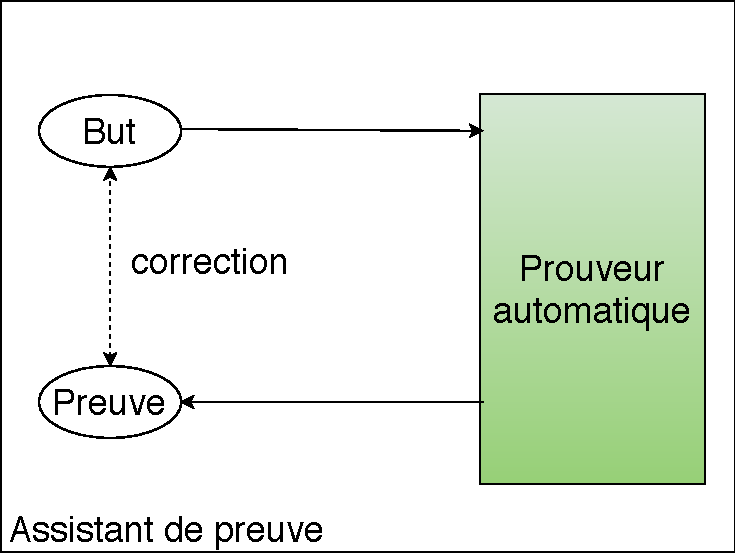
\includegraphics[height=5cm]{1_Autarcique.pdf}\\
Approche sceptique\\
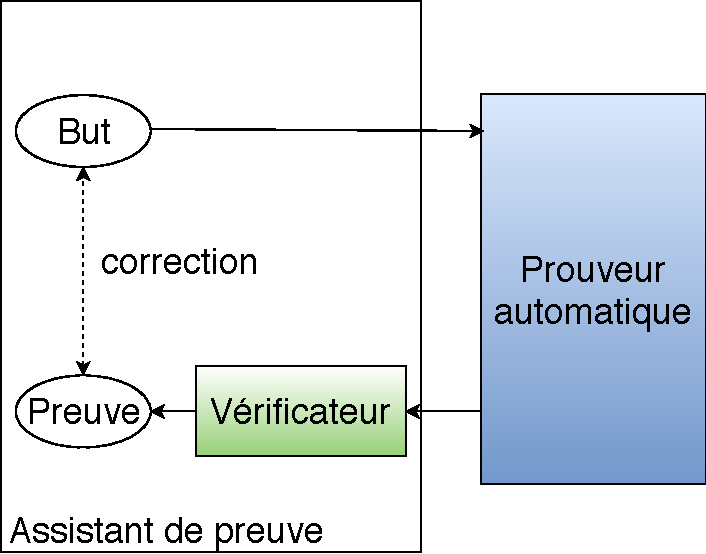
\includegraphics[height=5cm]{2_Sceptique.pdf}\\

\end{center}
\end{multicols}

L'approche autarcique consiste à vérifier le code du prouveur automatique à l'intérieur de l'assistant de preuve. L'avantage de cette méthode est qu'une fois cette vérification faite, on sait que chaque appel du prouveur automatique nous renverra une preuve correcte. \\

Dans l'approche sceptique, le certificat renvoyé par le prouveur automatique est vérifié à chaque appel de celui-ci. Cette approche, utilisée par SMTCoq, ne permet pas de garantir la complétude du système: certains buts valides ne sont pas démontrés, notamment lorsque le prouveur automatique renvoie un certificat erroné ou que la reconstruction de la preuve par SMTCoq n'est pas possible. En retour, cette approche ne fige pas l'implantation du prouveur automatique puisque ce n'est pas son code qui est vérifié mais sa réponse. Un autre avantage est que l'effort de certification est plus restreint: pour un certificat fixé, il faut vérifier que celui-ci correspond bien à une preuve du but.

\subsection{Fonctionnement de SMTCoq}

\subsubsection{Amélioration de l'automatisation}\label{negation}

Chacune des tactiques Coq définies par SMTCoq invoque un prouveur automatique différent: zChaff, CVC4 ou veriT. Ces tactiques permettent à l'utilisateur Coq de faire appel à un prouveur automatique pour résoudre le but courant et donc de profiter de l'automatisation du prouveur. \\

Les prouveurs automatiques fournissent un certificat uniquement dans le cas où le problème n'est pas satisfiable (\ref{sortie}). Pour utiliser ce fonctionnement, SMTCoq envoie la négation du but au prouveur automatique. La preuve ne peut être reconstruite que dans le cas où la réponse est $unsat$ et est accompagnée d'un fichier de certificat. Ce fichier prouve que la négation du but mène à l'absurde. Autrement dit, on obtient une preuve de la double négation du but. Les domaines des variables étant toujours supposés décidables dans SMTCoq, on récupère une preuve du but initial.

\begin{center}
    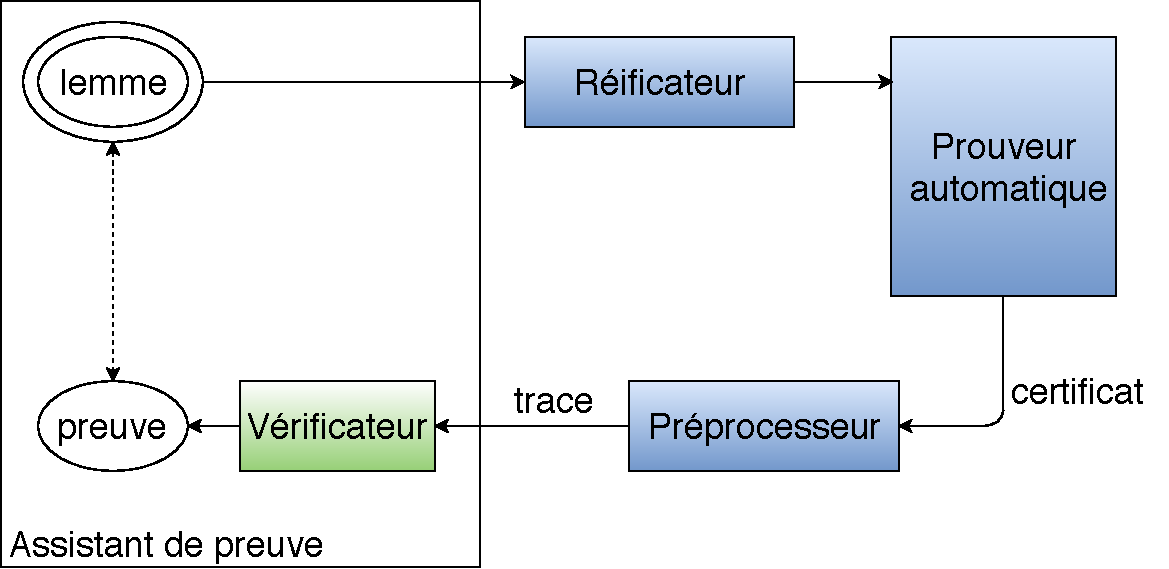
\includegraphics[height=5cm]{Automatisation.pdf}
\end{center}

La première étape est la réification, le lemme est traduit dans l'AST des formules acceptées par SMTCoq. Le prouveur automatique est appelé à partir de cet AST. En cas de succès de ce prouveur, on obtient un certificat de preuve. 
Il s'agit ensuite de rejouer ce certificat en Coq, on utilise pour cela le vérificateur de SMTCoq. Il faut donc mettre le certificat dans une forme adaptée qu'on appelle trace. Le préprocesseur effectue une étape de \textit{parsing} du certificat qui se souvient des sous-formules déjà rencontrées (\textit{hash-consing}) à l'aide de tables de hachage.  Il y a aussi une étape d'adaptation de ces certificats. En effet, les prouveurs automatiques peuvent parfois ne pas mentionner une étape de la preuve qu'il faut alors construire. De plus, il faut pouvoir adapter les certificats fournis par le prouveur automatiques qui peuvent reposer sur une logique différente de celle de Coq (???). 


\subsubsection{Amélioration de la confiance} \label{confiance}

Dans la suite on s'attachera principalement à développer l'aspect automatisation de Coq mais SMTCoq propose également une commande de reconstruction d'une preuve effectuée par un prouveur automatique.

\begin{center}
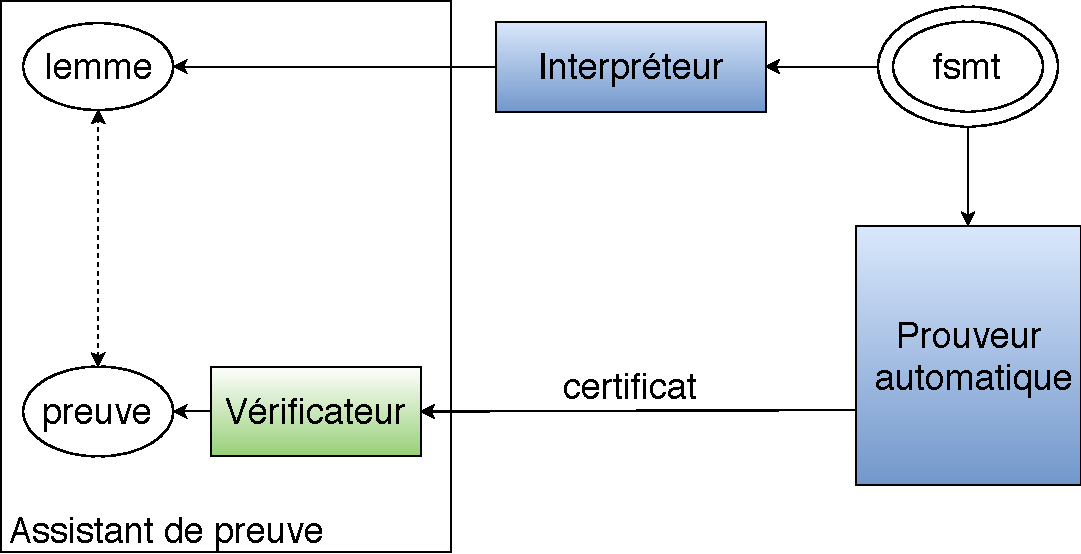
\includegraphics[height=5cm]{Confiance.pdf}
\end{center}

Cette commande prend en paramètre un fichier 'fsmt' décrivant le lemme (typiquement écrit en SMT-LIB) et le certificat fourni par un prouveur automatique. Le lemme Coq est reconstruit à l'aide de l'interpréteur de SMTCoq et la preuve est reconstruite grâce au vérificateur. Une fois la reconstruction faite, la vérification que la preuve correspond bien au lemme est laissée à Coq. \\

Puisqu'un nouveau lemme Coq est créé, l'utilisateur peut vérifier que c'est bien le but qu'il voulait prouver. Ainsi, la confiance dans les prouveurs automatiques est améliorée: on peut vérifier la réponse du prouveur.


\subsubsection{Cas d'application de SMTCoq}

Dans les deux cas, les formules acceptées sont les formules logiques propositionnelles en forme prénexe. Les domaines de quantification doivent aussi être décidables. La logique est étendue avec les combinaisons des théories suivantes: arithmétique linéaire sur $\mathbb{Z}$, égalité et fonctions non-interprétées, auxquelles s'ajouteront la théorie des vecteurs de bits et la théorie des tableaux. 

\subsection{Utilisation de SMTCoq}

\subsubsection{La tactique $verit$}

La nouvelle tactique $verit$ définie par SMTCoq permet de résoudre automatiquement les buts dans les booléens en forme prénexe. On reprend l'exemple de la partie \ref{fonctionnement_prouveurs}.

\begin{lstlisting}[frame=single]
Lemma lia5 : 
  forall x y,
    negb ( ((x+y <=? - (3)) && (y >=? 0) || (x <=? - (3))) && (x >=? 0)).
Proof.
    verit.
Qed.
\end{lstlisting}

La tactique commence par introduire les variables quantifiées universellement en tête de formule (ici c'est $x$ et $y$) puis s'attend à ne pas avoir d'autres quantificateurs. C'est ensuite la négation de la formule qui est envoyée à veriT. La reconstruction de la preuve ne peut avoir lieu que si veriT renvoie $unsat$ ainsi qu'un fichier de certificat.

\subsubsection{La commande de reconstruction}

La commande $Verit\_Theorem$ nous permet de créer un terme Coq à partir du certificat fourni par veriT appelé sur $lia5.smt2$. On obtient alors le terme Coq $lia5$: \\

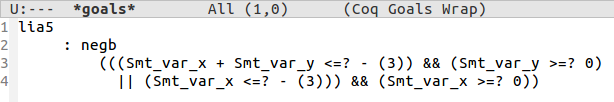
\includegraphics[height=2cm]{checklia5.png}

On notera que c'est bien la négation de la formule énoncée dans le fichier SMT-LIB. 



\section{Transformation de certificats}

Nous avons vu dans la partie précédente que c'est grâce à un procédé de réification (\ref{reification}) que l'on peut passer du but initial en Coq au prouveur automatique. Nous allons maintenant voir comment la réponse du prouveur automatique, le fichier de certificat, peut être transformée en un terme de preuve Coq.

\subsection{Des certificats de toutes les couleurs} \label{des_certificats}

La tactique $verit$ interprète le fichier de certificat \textit{tcertif} fourni par le prouveur automatique en un terme Coq \textit{ccertif}, ce qui permet de construire une preuve du but initial. \\

\begin{center}
\begin{tabular}{ |c||c|c|c| } 
 \hline
 Format & Fichier texte & Code Ocaml & Code Coq \\ 
 \hline
 Appellation & \textit{tcertif} & \textit{ocertif} & \textit{ccertif} \\ 
 \hline
 Composant & \textit{trule} & \textit{orule} & \textit{crule} \\ 
 \hline
\end{tabular}
\end{center}

Cette interprétation passe par une étape intermédiaire \textit{ocertif} écrite en Ocaml. Cette étape a plusieurs avantages. En premier lieu, elle permet d'utiliser les outils de \textit{parsing} du fichier de certificat (ocamllex, ocamlyacc). Par ailleurs, en utilisant la représentation Ocaml des termes Coq, la traduction d'un \textit{ocertif} en un \textit{ccertif} est facilitée. Enfin, les \textit{ocertif} sont définis dans un format facilement manipulable ce qui permet d'appliquer des adaptations (\ref{processing_forallinst}), des simplifications (\ref{regroupement}) ou encore des optimisations (\ref{alloc}).

\subsection{Transformation de Tseitin et \textit{hash-consing}} \label{tseitin}

\subsubsection{Motivations}

La transformation de Tseitin d'une formule donne une formule équisatisfiable qui est en CNF. L'avantage de cette transformation est que sa complexité est linéaire en temps comme en espace. En comparaison, l'utilisation des lois de De Morgan pour obtenir une formule en CNF a une complexité en pire cas exponentielle. Le principe de cette transformation est d'introduire de nouvelles variables pour toutes les sous-formules, ce qui correspond au \textit{hash-consing} qui est fait par SMTCoq. Cette étape intervient au moment du \textit{parsing}, c'est-à-dire au moment du passage d'un \textit{tcertif} à un \textit{ocertif}. Du point de vue de SMTCoq, ce procédé signifie un gain en espace (les sous-formules ne sont pas répétées) et un gain en temps (les comparaisons de formules deviennent des comparaisons d'entiers).


\subsubsection{Fonctionnement}

La transformation commence par nommer toutes les sous-formules en partant des feuilles. La nouvelle formule à satisfaire est alors la conjonction de la variable représentant toute la formule et de formules additionnelles qui garantissent que les nouvelles variables sont équivalentes aux sous-formules qu'elles représentent. \\

On reprend l'exemple de la partie \ref{fonctionnement_prouveurs}. En nommant les atomes on avait obtenu la formule $((a \wedge b) \vee c) \wedge d$. On introduit également $e$ pour la sous-formule $a \wedge b$, $f$ pour la sous-formule $e \vee c$ et $g$ pour la sous-formule $f \wedge d$ qui est en fait toute la formule. La formule transformée devient donc $g \wedge D_e \wedge D_f \wedge D_g$ où les $D_\alpha$ sont des formules qui nous assurent que $\alpha$ est équivalent à la formule qu'il représente. On a par exemple $D_e = (\neg a \vee \neg b \vee e) \wedge (\neg e \vee a) \wedge (\neg e \wedge b)$. \\

Dans SMTCoq, au lieu de rajouter les formules $D_\alpha$, les sous-formules sont enregistrées dans un tableau: une nouvelle sous-formule peut faire référence à une sous-formule qui est à un indice précédent dans le tableau. 

\subsection{Le vérificateur}

Le vérificateur définit en Coq un type \textit{crule} qui représente les \textit{trule} ainsi qu'une fonction $checker$. Nous allons définir ces termes, voir comment ils implémentent la sémantique des certificats de veriT (\ref{sortie}) et comment ils sont utilisés pour produire le terme de preuve.


\subsubsection{Le type inductif \textit{crule}}\label{regroupement}


Une \textit{crule} est un type somme (???), chaque constructeur pouvant représenter alternativement l'une ou l'autre d'un ensemble de \textit{trule}. Le constructeur $Res$ ne représente que la règle $resolution$ mais d'autres constructeurs peuvent représenter différentes règles en fonction de leurs paramètres. Par exemple, le constructeur $ImmBuildProj$ regroupe les règles $not\_implies0$ et $not\_implies1$ et contient aussi un paramètre de type \textit{int} qui vaut $0$ ou $1$ et qui indique quelle est la \textit{trule} représentée. Ce regroupement permet d'unifier le fonctionnement de règles similaires et donc de simplifier le traitement de ces règles dans la suite du code. \\

On appellera \textit{ccertif} la liste de toutes les \textit{crule} du certificat.


\subsubsection{La fonction récursive $checker$} \label{checker}

Pour enregistrer le résultat des règles précédentes on utilise un tableau de clauses appelé état. On rappelle qu'une clause représente la disjonction d'une liste de formules. On notera $(f_1 \,\, f_2\,\,  ... \,\, f_n)$ la clause contenant les formules $f_1$, $f_2$, ..., $f_n$. La fonction $checker$ implémente l'application des règles du certificat et modifie donc l'état à chaque nouvelle \textit{crule} rencontrée. Plus précisément, $checker$ est une fonction Coq qui est définie récursivement sur son paramètre de type \textit{ccertif} et qui a aussi un paramètre état. À chaque appel de $checker$, une nouvelle \textit{crule} $cr$ est consommée, $checker$ met alors à jour l'état courant en fonction de $cr$.\\

Il n'y a pas de \textit{crule} correspondant à la règle $input$. À la place, le tableau d'état est initialisé avec le résultat de la règle $input$. Ce fonctionnement n'est possible que lorsqu'il n'y a qu'un seul $input$, ce qui est le cas de la tactique $verit$ (la valeur d'initialisation est la négation du but). La taille du tableau est égale au nombre de règles du \textit{tcertif}. \\

Lorsque toute la liste \textit{ccertif} a été consommée, $checker$ renvoie $true$ si la dernière case du tableau d'état contient la clause vide et $false$ sinon.

\subsubsection{Théorème de correction}

Le type des formules est réifié et on peut définir une fonction d'évaluation $evaluation$ qui inverse la réification (\ref{interet_reification}). Le vérificateur repose sur le théorème de correction qui nous assure que pour tout \textit{ccertif} $cc$ et toute formule $f$, si le tableau d'état $t$ est initialisé comme décrit précédemment, alors: 
\[ checker  \,\, cc \,\, t \, = \, true \quad \Rightarrow \quad \neg (evaluation \, \, f) \]
Une fois celui-ci démontré, la preuve est obtenue en l'appliquant à la réflexivité de l'égalité. En effet, si $checker  \,\, cc\,\, t  $ est convertible à $true$, alors $checker  \,\, cc\,\, t = true $ est convertible à $true = true$.

\subsubsection{Preuve du théorème de correction} \label{preuve_correction}

On dit qu'une clause est valide lorsque son évaluation est prouvable. La preuve du théorème de correction repose sur le lemme $step\_checker\_correct$ qui s'énonce ainsi: si toutes les clauses du tableau d'état sont valides alors une étape de $checker$ modifie ce tableau en un tableau dont toutes les clauses sont valides. Il suffit en fait de vérifier que la nouvelle clause générée par $checker$ est valide. \\ 

À partir de ce lemme on obtient une preuve du théorème de correction. Supposons que le lemme initial (la négation du but dans le cas de la tactique $verit$) soit prouvable. Initialement, le tableau d'état ne contient donc que des clauses valides et, d'après $step\_checker\_correct$, cette propriété est conservée par la fonction $checker$. Si  de plus $checker$ renvoie $true$ cela veut dire qu'il y a la clause vide dans le dernier tableau d'état. L'interprétation de la clause vide nous conduit à une contradiction.


\subsubsection{Exemple de l'identité}

Considérons le but Coq suivant où $implb$ est l'implication booléenne:
\begin{lstlisting}[frame=single]
  Lemma identity A : implb A A.
\end{lstlisting}  
Lorsqu'on applique $verit$, puisque c'est la négation du but qui est envoyée, le prouveur automatique nous renvoie le \textit{tcertif} de \ref{not_implies}. Celui-ci est traduit par SMTCoq en un \textit{ccertif} $cc$ et l'état est initialisé en un tableau $t$: 
$cc = [ImmBuildProj \,\, 0 \,\, 0; \,ImmBuildProj \,\, 1 \,\, 0; \, Res \,\, 1 \,\, 2] $ et $t = [|nid; nid; nid; nid|]$ où $nid$ est la clause $( \neg (A \Rightarrow A))$.
\begin{align*}
    checker \,\, cc \,\, t &\equiv checker \,\, [ImmBuildProj \,\, 0 \,\, 0; \,ImmBuildProj \,\, 1 \,\, 0; \, Res \,\, 1 \,\, 2] \,\, [| nid; nid; nid; nid|] \\
    &\equiv checker \,\, [ImmBuildProj \,\, 1 \,\, 0; \, Res \,\, 1 \,\, 2] \,\, [| nid; (A); nid; nid|] \\
    &\equiv checker \,\, [Res \,\, 1 \,\, 2] \,\, [| nid; (A); (\neg A); nid|] \\
    &\equiv checker \,\, [] \,\, [| nid; (A); (\neg A); ()|] \\
    &\equiv true
\end{align*}
En appliquant le théorème de correction, on obtient $\neg (evaluation (\neg (A \Rightarrow A)))$, soit $\neg \neg (implb\,\, A \,\,A)$. On a vu que (\ref{negation}), dans le cadre de SMTCoq, on peut alors obtenir $implb \,\, A \,\, A$.

\subsection{Le préprocesseur}

Les avantages d'une étape intermédiaire de compilation des certificats sont multiples (\ref{des_certificats}). Nous détaillons le format utilisé puis nous donnons une optimisation rendue possible par cette étape.

\subsubsection{Le type Ocaml \textit{orule}}

 Les \textit{orule} sont des enregistrements constitués, en plus du code Ocaml d'une \textit{crule}, de méta-données qui permettent leur modification. En particulier, les \textit{orule} contiennent un champ $prev$ et un champ $next$. Ainsi, un \textit{ocertif} est une liste doublement chaînée de \textit{orule}. Les \textit{orule} contiennent aussi un champ $used$ de type \textit{int} qui est utilisé par la fonction $alloc$.


\subsubsection{Allocation dans le tableau état} \label{alloc}

On remarque que dans l'exemple précédent, le tableau d'état n'a pas besoin d'être aussi grand: 2 emplacements suffisent pour ce certificat. Pour réduire l'espace mémoire utilisé, il faut calculer le nombre maximum de clauses à retenir à chaque étape du $checker$, c'est ce que fait la fonction $alloc$. La taille du tableau d'état est fixée à cette valeur. Cette fonction assigne aussi une position dans un nouveau paramètre des \textit{orule}. Nous noterons ce paramètre de position au début, de sorte que lorsque $checker$ rencontre la \textit{crule} $ImmBuildProj \,\, 0\,\, 1 \,\, 2$, la case $0$ de l'état est modifiée en $\neg Y$ si la case $2$ de l'état contient $\neg(X \Rightarrow Y)$. Puisque les emplacements des clauses sont modifiés, il faut aussi modifier les dépendances des règles. Enfin, $checker$ prend un paramètre qui indique quelle est la position de la dernière règle, le résultat de la dernière règle n'étant pas nécessairement au dernier emplacement du tableau d'état.  
\begin{align*}
    checker \,\, cc \,\, t \,\, 0 &\equiv checker \,\, [ImmBuildProj \,\, 0\,\, 0 \,\, 0; \,ImmBuildProj \,\, 1\,\, 1 \,\, 1; \, Res \,\, 0 \,\, 0 \,\, 1] \,\, [| nid; nid|] \,\, 0 \\
    &\equiv checker \,\, [ImmBuildProj \,\, 1 \,\, 1 \,\, 1; \, Res \,\, 0 \,\, 0 \,\, 1] \,\, [| (A); nid|] \,\, 0 \\
    &\equiv checker \,\, [Res \,\, 0 \,\, 0 \,\, 1] \,\, [| (A); (\neg A)|] \,\, 0 \\
    &\equiv checker \,\, [] \,\, [| (); (\neg A)|] \,\, 0 \\
    &\equiv true
\end{align*}


\section{Préprocesseur pour les lemmes quantifiés}

Dans cette partie on commence par donner la forme générale des certificats de veriT dans le cas des lemmes quantifiés universellement. On explique ensuite comment un certificat peut être modifié pour faciliter son encodage en un \textit{ccertif} (partie \ref{instanciations}). \\

Nous étudierons l'exemple de la proposition Coq suivante: 

\begin{lstlisting}[frame=single]
Lemma instance_2 f : 
  (forall x, f (x+1) =? f x + 7) ->
  f 3 =? f 2 + 7.
\end{lstlisting}


\subsection{Instanciation d'un lemme par veriT: la règle $forall\_inst$}

Lorsqu'un lemme en forme prénexe est donné par une règle $input$, veriT peut instancier ce lemme avec la règle $forall\_inst$. Donnons le début du certificat simplifié obtenu en appelant $verit$ sur l'exemple:
\begin{align*}
0&:(input \,\,(forall\,\, x,\,\, f (x+1) = f(x)+7) \\
1&:(forall\_inst \,\,((not \,\,(forall\,\, x, \,\,f (x+1) = f(x)+7)) \,\,(f (2+1) = f(2)+7)) )\\
2&:(resolution  \,\, (f (2+1) = f(2)+7) \,\,1 \,\,0) 
\end{align*}
On remarquera que la règle $forall\_inst$ ne dépend d'aucune autre règle et que l'utilisation de son résultat passe une règle $resolution$.

\subsection{Lier une instanciation à un lemme} \label{lien}

\subsubsection{Lien entre une règle $forall\_inst$ et une règle $input$} 

Dans l'exemple, la dépendance de la règle $forall\_inst$ au lemme donné dans la règle $input$ est évidente pour plusieurs raisons: le certificat est de petite taille, il y a égalité syntaxique entre le lemme et une sous-formule du résultat de la règle $forall\_inst$, la règle de résolution qui utilise la règle $forall\_inst$ est située juste juste après celle-ci et a exactement 2 dépendances. Cependant, dans le cas général, aucune de ces raisons ne reste valide. En particulier, veriT fait un renommage des variables liées qui apparaissent dans les lemmes (l'exemple complet est présenté dans l'annexe B). Retrouver la dépendance demande donc, a priori, d'unifier à $\alpha$-équivalence près des formules contenues dans une règle $forall\_inst$ et dans les règles $input$. Heureusement, veriT fait un \textit{hash-consing} des formules qui apparaissent dans les \textit{tcertif}. Cela nous permet d'enregistrer la dépendance au lemme dans la règle $forall\_inst$ au moment du \textit{parsing} des certificats de veriT. La règle $1$ devient: 
\begin{align*}
1:(forall\_inst \,\, ((not \,\,(forall \,\,x, \,\,f (x+1) = f(x)+7)) \,\,(f (3) = f(2)+7))) \,\,0) 
\end{align*}

\subsubsection{Lien entre une formule et un lemme Coq}


-lemme coq donné par l'utilisateur\\
-le problème vient du fait que les lemmes peuvent être modifiés par veriT (en particulier la symétrie de l'égalité), que le but initial doit être fidèlement traduit pour qu'on ait bien le fait que l'interprétation de la réification d'un terme soit égale au terme \\
-pour faire ça on utilise deux tables de hachage distinctes. Une pour stocker les lemmes exactement comme ils apparaissent dans verit afin de prouver la bonne chose. Une autre pour les reconnaître une fois qu'ils apparaissent\\
-une fois que c'est fait on peut reconnaître les lemmes et en particulier il faut distinguer le but des autres lemmes (pas le même traitement du tout)\\
-d'autre part le hash-consing 'tel quel' ne doit se faire que sur les termes qui ne contiennent pas de variable liées pour ne pas encombrer les tables de hachage de symboles inutiles\\
-combiner les 2 liens


\subsection{Logique de veriT et de Coq}
On a vu que veriT utilise des clauses de la forme: 
\[  \neg (\forall \, x, \, P(x)) \vee (P \, (n)) \]

Une telle clause est une tautologie pour tout prédicat $P$ et toute valeur $n$ en logique classique. \\

Cependant, dans la logique intuitionniste de Coq, ce n'est plus vrai. Une solution serait de remplacer cette clause par la formule:

\[   (\forall \, x, \, P(x)) \Rightarrow (P \, (n)) \]
mais cela demande de profonds changements des \textit{ccertif} et de leur utilisation par le vérificateur: 
\begin{itemize}

\item il faut créer une nouvelle \textit{crule} pour pouvoir prendre en compte toutes les règles $input$ et pas seulement celle correspondant au but comme c'est fait au moment de l'initialisation du tableau d'état (\ref{checker})
\item il faut modifier le format des \textit{crule} pour accepter les formules quantifiées ce qui demande ensuite de raisonner dans Coq sur des termes à $\alpha$-équivalence près.
\end{itemize}

\subsection{La règle $same$}

Il arrive que, à la suite de modifications des certificats, une règle devient inutile car son résultat est le même que celui d'une règle précédente. Pour la supprimer, il faut modifier tous les paramètres des règles suivantes pour qu'ils fassent référence à la première règle qui a ce même résultat. Cependant, faire cette modification à chaque fois que l'on veut supprimer une règle a une complexité quadratique en la taille des certificats. Pour remédier à ce problème, on introduit une nouvelle \textit{orule} $same$ qui est une règle qui dépend d'une seule autre règle. Dans un premier temps les règles à supprimer sont remplacées par des règles $same$ et un dictionnaire est créé afin d'associer à chaque règle $same$ la règle non-$same$ lui correspondant (associer une règle $same$ à sa dépendance retombe dans un comportement quadratique). Ensuite les règle $same$ sont supprimées et les paramètres des règles restantes sont modifiés en suivant le dictionnaire.

\subsection{Modifier le résultat de la règle $forall\_inst$} \label{processing_forallinst}

Pour ces raisons, il est préférable de modifier les règles de la forme:
\[id:(forall\_inst \,\,((not \,\,lemma) \,\,lemma\_inst) \,\,id\_lemma)\]
où $lemma$ est un des lemmes rajoutés par l'utilisateur et $lemma\_inst$ est une instance de ce même lemme en une règle:
\[id:(forall\_inst \,\,(lemma\_inst) \,\, id\_lemma)\]

Il faut aussi modifier les règles suivantes qui dépendent du résultat de cette règle. On fait l'hypothèse supplémentaire qu'une règle $forall\_inst$ dépendant d'un lemme $l$ ne sera utilisée dans la suite du certificat que dans une règle de résolution ayant aussi une dépendance à $l$. On se ramène donc à modifier seulement les règles de résolution, ce que l'on fait ainsi: si une règle de résolution a pour liste de dépendance $dep$, on trouve toutes les règles $forall\_inst$ de cette liste et on enlève leurs dépendances de $dep$. Cette modification a un complexité en pire cas linéaire dans la taille des certificats. Dans le cas où il ne reste plus qu'une seule dépendance, la règle $resolution$ devient une règle $same$. En reprenant l'exemple de la section précédente, on obtient: 
\begin{align*}
0&:(input\,\, (forall \,\,x, \,\, f (x+1) = f(x) + 7)) \\
1&:(forall\_inst \,\,(f (2+1) = f(2) + 7) \,\,0) \\
2&:(same\,\, (f(2+1) = f(2) + 7) \,\,1) 
\end{align*}


\section{Vérificateur pour les lemmes quantifiés} \label{instanciations}

Pour traiter le cas des lemmes rajoutés au contexte par l'utilisateur, on a besoin de rajouter un constructeur au type \textit{crule}. On verra comment modifier le vérificateur en conséquence afin de rétablir la preuve de correction et de préserver l'automatisation de SMTCoq.


\subsection{La \textit{crule} $Forallinst$}

Rajouter un constructeur au type \textit{crule} demande de compléter la preuve de  $step\_checker\_correct$ correspondant à cette nouvelle règle (\ref{preuve_correction}). Le reste de la preuve de correction ne dépendant pas des \textit{crule} autrement que par ce lemme, c'est la seule modification à apporter à la preuve quand on ajoute une nouvelle règle. C'est un autre aspect de la modularité de SMTCoq. \\

Le nouveau constructeur s'écrit $Forallinst\,\, p\,\, lemma\,\, plemma \,\,lemma\_inst \,\,pinstanc$ où $p$ est le paramètre de position (\ref{alloc}), $lemma$ est le lemme dont on a identifié la dépendance (\ref{lien}), $plemma$ est la preuve de ce lemme, $lemma\_inst$ est l'instanciation et $pinstanc$ est un élément du type $lemma \rightarrow lemma\_inst$. \\

Une étape de la fonction $checker$ correspondant à une telle \textit{crule} modifie la clause $p$ de l'état en la clause $lemma\_inst$. On peut facilement prouver que $lemma\_inst$ est valide, et même indépendemment des clauses contenues par l'état. En effet, il suffit d'appliquer $pinstanc$ à $plemma$. On a donc rétabli la preuve du théorème de correction.\\

Le problème est en fait déplacé puisqu'il faut maintenant, pour construire une \textit{crule}, donner une preuve d'instanciation, c'est-à-dire une preuve le lemme implique l'instance. Cette preuve est donnée à l'aide d'un ``cut'' (tactique $assert$ en Coq), ce qui nous permet de donner les preuves d'instanciation dans un deuxième temps.

\subsection{Preuves d'instanciation}

La structure d'une instance peut différer de celle du lemme pour plusieurs raisons. Pour chacune de ces raisons nous verrons comment obtenir tout de même une preuve d'instanciation. Grâce à ces résultats on peut définir une tactique qui permet de trouver automatiquement n'importe quelle preuve d'instanciation (voir annexe C).

\subsubsection{Preuve automatique d'une instanciation}

Le lemme Coq suivant correspond directement à l'instanciation du lemme donnée :
\begin{lstlisting}[frame=single]
Lemma instance_c P (c : Z): 
  (forall x, P x) ->
  P c.
\end{lstlisting}

De tels but peuvent peuvent être prouvés automatiquement par la tactique $auto$. Cependant ce n'est plus le cas lorsque le but est légèrement modifié. Par exemple, le lemme suivant ne peut pas être prouvé directement par $auto$:

\begin{lstlisting}[frame=single]
Lemma instance_3 f (c : Z): 
  (forall x, f x =? f c) ->
  f c =? f 3.
\end{lstlisting}
Il faut donc remettre le but dans une forme qui correspond à celle du lemme. Dans le dernier cas il s'agit de réécrire le lemme $Z.eqb\_sym$ avant d'appliquer la tactique $auto$.

\subsubsection{Transformation $impl\_split$}

Lorsque qu'un lemme est de la forme:
\[ id1:(input \,\,(forall\,\, x,\,\, f \,\,x \Rightarrow b)) \]
la \textit{trule} $forall\_inst$ peut être:
\[ id2:(forall\_inst \,\, ( (not\,\, (forall\,\, x, \,\,f \,\, x \Rightarrow b)) \,\,(or \,\,(not \,\,(f\,\, c)) \,\, b))) \]
au lieu de la \textit{trule} attendue:
\[ id2:(forall\_inst  \,\,( (not \,\,(forall \,\,x,\,\, f\,\, x \Rightarrow b))\,\, (f \,\,c \Rightarrow b))) \]

Cette différence se retrouve directement dans la preuve d'instanciation associée et peut être résolue en ajoutant un lemme à la base de lemmes $Resolve$. La tactique $auto$, qui utilise cette base de lemme, trouvera automatiquement la preuve pour ce type de différence entre lemme et instance.

\begin{lstlisting}[frame=single]
Lemma impl_split a b:
  implb a b -> orb (negb a) b.
Proof. intro. destruct a; destruct b; trivial. Qed.

Hint Resolve impl_split.
\end{lstlisting}

\subsubsection{Transformations liées à la symétrie de l'égalité}

A FAIRE : d'où ça vient? \\

Pour résoudre ce problème, on commence par remarquer que la plupart du temps lorsqu'une égalité est inversée alors elle le sont toutes. On écrit une tactique qui inverse toutes les égalités et pour chaque cas on essaye de résoudre le but en utilisant cette tactique et en ne l'utilisant pas.

\section{Utilisation de la tactique $verit$ avec des lemmes}

Add\_lemmas H1 ... Hn. \\
Clear\_lemmas.\\

verit\_base H1 .. Hn; vauto. \\
verit == (vbase avec n=0)\\

Exemple de la formalisation des listes d'entiers


\section{Travaux connexes et conclusion}

Ce stage s'inscrit dans une approche automatique de la démonstration dans un assistant de preuve et porte plus précisément sur SMTCoq. D'autres outils sont disponibles dans ce cadre, à commencer par Coqhammer \cite{coqhammer} qui est aussi un \textit{plugin} pour Coq qui utilise des prouveurs automatiques. À la différence de SMTCoq, lors de la reconstruction de la preuve, Coqhammer liste les lemmes qui apparaissent dans le certificat et n'utilise rien d'autre que cette liste du certificat. Ainsi, il y a une recherche qui est faite par des tactiques en Coq et qui permet de retrouver la preuve. Cette méthode est plus robuste que celle  de SMTCoq vis-à-vis des prouveurs automatiques mais demande de chercher à nouveau la preuve et est donc plus coûteuse. De la même manière, pour retrouver les instanciations des lemmes (partie \ref{instanciations}), la recherche a été faite en Coq. Cette méthode s'est avérée utile pour passer outre certaines simplifications silencieuses des certificats qui apparaissent à ce niveau dans les certificats de veriT. Une autre différence est que SMTCoq propose aussi une commande de vérification ce qui permet d'améliorer la confiance accordée aux prouveurs automatiques (\ref{confiance}).\\
On peut aussi mentionner Sledgehammer \cite{sledgehammer_manual} qui est un outil développé pour l'assistant de preuve Isabelle afin d'y intégrer une interface sceptique avec des prouveurs automatiques. Sledgehammer a mis en place un sélectionneur de lemmes qui apprend quels lemmes il est judicieux d'envoyer aux prouveurs automatiques \cite{hol_selector}.\\

En résumé, ce stage a permis d'améliorer l'expressivité de SMTCoq tout en restant dans un cadre qui assure la correction de la méthode. Cette amélioration de l'expressivité a été confirmée par de nouveaux tests. Enfin, ce stage ouvre de nouvelles pistes de travail (\ref{persp}): améliorer l'efficacité, étendre les cas d'application, utiliser SMTCoq pour la certification Why3, etc.



\newpage
\pagestyle{empty}
\renewcommand\refname{Bibliographie}
\nocite{*}
\bibliography{biblio}{}
\bibliographystyle{plain}



\section*{Annexe A: Formules booléennes conjonctives}

On donne ici deux définitions, la preuve de leur équivalence, la mise en forme de peigne des formules conjonctives, la correction de cette fonction, la réification d'un booléen et une tactique qui utilise la réflexion calculatoire.

\begin{lstlisting}[frame=single]
Require Import Bool.

Inductive AndTree :=
  Bool (_ : bool)
| And (_ _: AndTree).

Inductive Evaluation : AndTree -> bool -> Prop :=
  EvalBool b :
    Evaluation (Bool b) b
| EvalAnd b1 b2 b3 t1 t2 :
    Evaluation t1 b1 -> Evaluation t2 b2 -> b1 && b2 = b3 ->
    Evaluation (And t1 t2) b3.

Definition t :=
  And (And (Bool true) (Bool false)) (And (Bool true) (Bool true)).

Lemma Eval_t_false : Evaluation t false.
Proof.
  eapply EvalAnd ; [
    eapply EvalAnd ; [ apply EvalBool | apply EvalBool | reflexivity ]
  | eapply EvalAnd ; [ apply EvalBool | apply EvalBool | reflexivity ]
  | reflexivity ].
Qed.

Fixpoint evaluation (t : AndTree) :=
  match t with
    Bool n => n
  | And t1 t2 => evaluation t1 && evaluation t2
  end.

Proposition Eval_eq_eval t b :
  Evaluation t b <-> evaluation t = b.
Proof.  
  revert b. induction t as [a | t1 IHt1 t2 IHt2]; simpl; intro b.
  -split; intro H.
   +now inversion H.
   +rewrite H. apply EvalBool.
  -split; intro H.
   +inversion H.
    apply IHt1 in H2; rewrite H2.
    now apply IHt2 in H3; rewrite H3.
   +eapply EvalAnd. now apply IHt1.
    now apply IHt2. assumption.
Qed.
   
Lemma eval_t_false : evaluation t = false.
Proof.
  reflexivity.
Qed.

Fixpoint append t1 t2 :=
  match t1 with
  | Bool n => And t1 t2
  | And t11 t12 => append t11 (append t12 t2)
  end. 

Fixpoint peigne (t : AndTree) :=
  match t with
  | Bool n => t
  | And t1 t2 => let pt1 := peigne t1 in
                 let pt2 := peigne t2 in
                 append pt1 pt2
  end.

Inductive eqt : AndTree -> AndTree -> Prop :=
  refl t: eqt t t
| sym t1 t2: eqt t1 t2 -> eqt t2 t1
| assoc t1 t2 t3: eqt (And t1 (And t2 t3)) (And (And t1 t2) t3)
| congru ta1 ta2 tb1 tb2: eqt ta1 tb1 -> eqt ta2 tb2 ->
                           eqt (And ta1 ta2) (And tb1 tb2)
| trans t1 t2 t3: eqt t1 t2 -> eqt t2 t3 -> eqt t1 t3.

Lemma eqt_correct t1 t2:
  eqt t1 t2 -> evaluation t1 = evaluation t2.
Proof.
  intro eq12. induction eq12; simpl.
  -reflexivity.
  -auto.
  -apply andb_assoc.
  -rewrite IHeq12_1.
   now rewrite IHeq12_2.
  -now rewrite IHeq12_1.
Qed.

Lemma append_eqt t1 t2:
  eqt (append t1 t2) (And t1 t2).
Proof.
  revert t2. induction t1; intro t2; simpl.
  -apply refl.
  -eapply trans. apply IHt1_1. eapply trans. eapply congru.
   apply refl. apply IHt1_2. apply assoc.
Qed.

Lemma peigne_eqt t:
  eqt (peigne t) t.
Proof.
  induction t; simpl.
  -apply refl.
  -eapply trans. apply append_eqt. now apply congru.
Qed.

Lemma peigne_correct t:
  evaluation (peigne t) = evaluation t.
Proof.
  apply eqt_correct. now apply peigne_eqt.
Qed. 

Ltac reify A :=  match A with
  | andb ?X ?Y => let rx := reify X in
                  let ry := reify Y in
                  constr:(And rx ry)
  | ?X => constr:(Bool X) end.

Ltac peignify :=
  match goal with
  | [ |- ?A = ?B] =>
    let a := reify A in
    let b := reify B in
    change A with (evaluation a);
    change B with (evaluation b);
    rewrite <- (peigne_correct a);
    rewrite <- (peigne_correct b);
    simpl
  end.

Lemma peigne4 b1 b2 b3 b4:
  (b1 && b2) && (b3 && b4) = b1 && ((b2 && b3) && b4).
Proof.
   peignify. reflexivity.
Qed.
\end{lstlisting}

\section*{Annexe B: Fichier SMT-LIB et certificat veriT d'une instanciation}

\lstset{language=Java}

Lorsqu'on appelle veriT sur le fichier SMT-LIB $simple\_instance.smt2$ suivant: 
\begin{lstlisting}[frame=single]
(set-logic UFLIA)
(declare-fun f (Int) Int)
(assert (not (= (f 3) (+ (f 2) 7))))
(assert (forall ( (x Int) ) (= (f (+ x 1)) (+ (f x) 7))))
(check-sat)
(exit)
\end{lstlisting}

on obtient $unsat$ et la preuve dans un fichier contenant: 

\begin{lstlisting}[frame=single]
1:(input ((not #1:(= #2:(f 3) #3:(+ #4:(f 2) 7)))))
2:(input (#5:(forall ( (x Int) ) #6:(= #7:(f #8:(+ x 1)) #9:(+ #10:(f x) 7)))))
3:(tmp_betared (#11:(forall ( (@vr0 Int) ) #12:(= #13:(f #14:(+ @vr0 1)) #15:(+ #16:(f @vr0) 7)))) 2)
4:(tmp_qnt_tidy (#17:(forall ( (@vr1 Int) ) #18:(= #19:(f #20:(+ @vr1 1)) #21:(+ #22:(f @vr1) 7)))) 3)
5:(forall_inst (#23:(or (not #17) #24:(= #3 #25:(f #26:(+ 2 1))))))
6:(or ((not #17) #24) 5)
7:(resolution (#24) 6 4)
8:(eq_transitive ((not #27:(= #2 #25)) (not #24) #1))
9:(eq_congruent ((not #28:(= 3 #26)) #27))
10:(resolution ((not #24) #1 (not #28)) 8 9)
11:(resolution ((not #28)) 10 1 7)
12:(la_disequality (#29:(or #28 (not #30:(<= 3 #26)) (not #31:(<= #26 3)))))
13:(or (#28 (not #30) (not #31)) 12)
14:(resolution ((not #30) (not #31)) 13 11)
15:(la_generic (#31))
16:(resolution ((not #30)) 14 15)
17:(la_generic (#30))
18:(resolution () 17 16)
\end{lstlisting}


\section*{Annexe C: Automatisation des preuves d'instanciation de lemmes}
\lstset{language=coq}
\begin{lstlisting}[frame=single]
Require Import SMTCoq Bool.
Open Scope Z_scope.

(* verit silently transforms an <implb a b> into a <or (not a) b> when
 instantiating a quantified theorem with <implb> *)
Lemma impl_split a b:
  implb a b = true -> orb (negb a) b = true.
Proof.
  intro H.
  destruct a; destruct b; trivial.
(* alternatively we could do <now verit_base H.> but it forces us to have veriT
   installed when we compile SMTCoq. *)
Qed.

Hint Resolve impl_split.

(* verit silently transforms an <implb (a || b) c> into a <or (not a) c> 
   or into a <or (not b) c> when instantiating such a quantified theorem *)
Lemma impl_or_split_right a b c:
  implb (a || b) c -> negb b || c.
Proof.
  intro H.
  destruct a; destruct c; intuition. 
Qed.

Lemma impl_or_split_left a b c:
  implb (a || b) c -> negb a || c.
Proof.
  intro H.
  destruct a; destruct c; intuition.
Qed.

(* verit considers equality modulo its symmetry, so we have to recover the
   right direction in the instances of the theorems *)
Definition hidden_eq a b := a =? b.
Ltac all_rew :=
  repeat match goal with
         | [ |- context [ ?A =? ?B]] =>
           change (A =? B) with (hidden_eq A B)
         end;
  repeat match goal with
         | [ |- context [ hidden_eq ?A ?B] ] =>
           replace (hidden_eq A B) with (B =? A);
           [ | now rewrite Z.eqb_sym]
         end.

(* An automatic tactic that takes into account all those transformations *)
Ltac vauto :=
  try (let H := fresh "H" in
       intro H; try (all_rew; apply H);
       match goal with
       | [ |- is_true (negb ?A || ?B) ] =>
         try (eapply impl_or_split_right; apply H);
         eapply impl_or_split_left; apply H
       end;
       apply H);
  auto.

Ltac verit :=
  verit_base; vauto.
\end{lstlisting}
\end{document}

